\section{Evaluation of main MPPT techniques\label{MPPTalgo}}

There are a variety of different techniques for finding the maximum power point. Therefore only three different methods are used in this thesis, otherwise it would go beyond the scope of this work. These three methods are the perturb and observe, constant voltage and incremental conductance. Perturb and observe and incremental conductance are the most used algorithms in commercial pv-panels. On the other hand, constant voltage has been selected as a comparison to methods that are not used so often. The reason for that is there other methods which are easier to implement but they have a high disadvantage.\todo{why as a comparison? AT}. 

\subsection{Constant voltage}
Empirical experiments have shown that the voltage of the MPP has a linear dependence on the open circuit voltage at different ambient conditions.

\begin{equation} \label{voltage_MPP}
V_{MPP} = k * V_{OC}	
\end{equation} 
In the equation \ref{voltage_MPP} k represents a constant that depends on the characteristics of the respective pv panel. To determine the value for k, the voltage for MPP and open circuit must be recorded for each temperature and solar irradiation. According to different papers, this value lies between 70 and 80 percent\cite{MPPTresearch}. The algorithm starts with the recording of the open circuit voltage and a predetermined k-value \todo{the k value is not detected... AT}. In each iteration step the $V_{MPP}$ is calculated first. After this, the operating voltage is compared with the calculated voltage of the MPP. If the voltage is not equal, the constant k is changed for the next iteration step to reach the MPP. When the algorithm has reached the MPP, the algorithm is stopped, as you can see in the flowchart in the figure \ref{fcconstantvoltage}\cite{flowchartVC}. \todo{how is the constant k calculated? I thought this method had a constant k determined by the characteristics of the pv, maybe im wrong but we should revise it. AT}

\begin{figure}[htbp]
	\begin{center}
		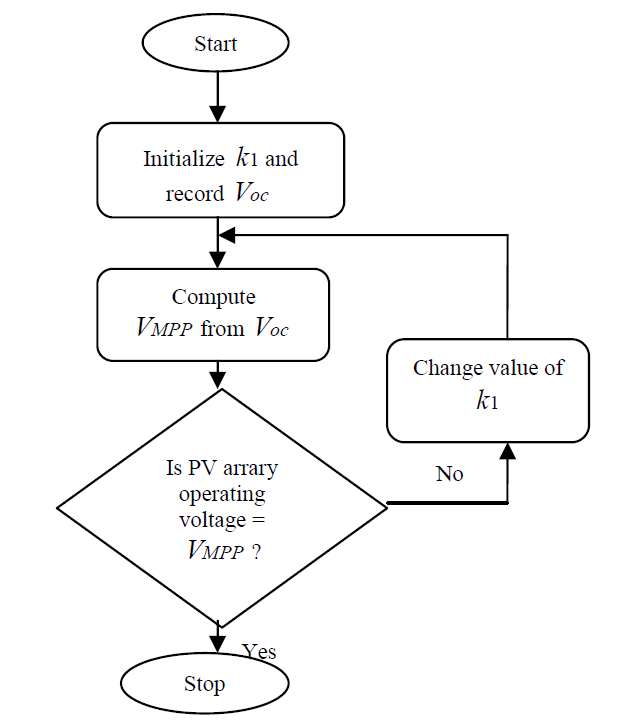
\includegraphics[width=0.5\textwidth]{../Pictures/P1/Flow_chart/Flow_chart_constant_voltage}
		\caption{flow chart constant voltage\cite{flowchartVC}. }
		\label{fcconstantvoltage}
	\end{center}	
\end{figure}

\subsection{Perturb and observe}
With the method "perturb and observe", the currently measured power is periodically compared with the previous power. If the measured power is greater than the power from the previous measurement, the voltage is further increased to reach the MPP. If a power reduction is detected after the comparison, the voltage is reduced \todo{this is not always true... depends on what side of the MPP we are working at. AT}. The flowchart in the figure \ref{fcperturbandobserve} illustrates this method. The classical algorithm uses a fixed step to change the voltage. When the MPP is reached, the algorithm oscillates around the MPP\cite{flowchartVC}. 

\begin{figure}[htbp]
	\begin{center}
		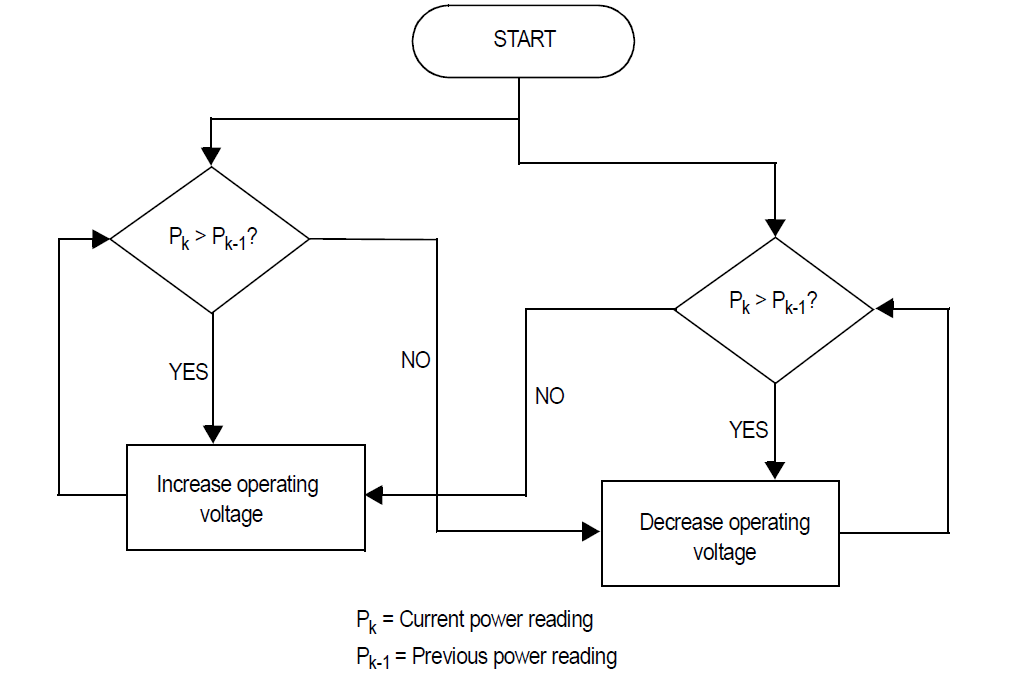
\includegraphics[width=0.7\textwidth]{../Pictures/P1/Flow_chart/flow_chart_perturb_observe}
		\caption{flow chart from perturb and observe\cite{AN1521_MC}.}
		\label{fcperturbandobserve}
	\end{center}	
\end{figure}

\subsection{Incremental conductancee}
The approach of incremental conductance is that the MPP is at the position where the derivative of the power with respect to the voltage is 0. On the left side of the MPP the derivative is greater than 0 while on the right side it is less than 0, this behavior is described by the following equations.\todo{I'll give you the equations later.}\newline
The algorithm compares the incremental conductance with the previous one to increase (left side of MPP) or decrease (right side of MPP) the voltage. After the MPP has been reached, the algorithm is stopped. Thus, there will be no oscillation around the MPP. If a change in the current is detected, the algorithm starts to find the MPP again, as you can see in the flowchart in the figure \ref{fcinccon}\cite{AN1521_MC}.
\begin{figure}[H]
	\begin{center}
		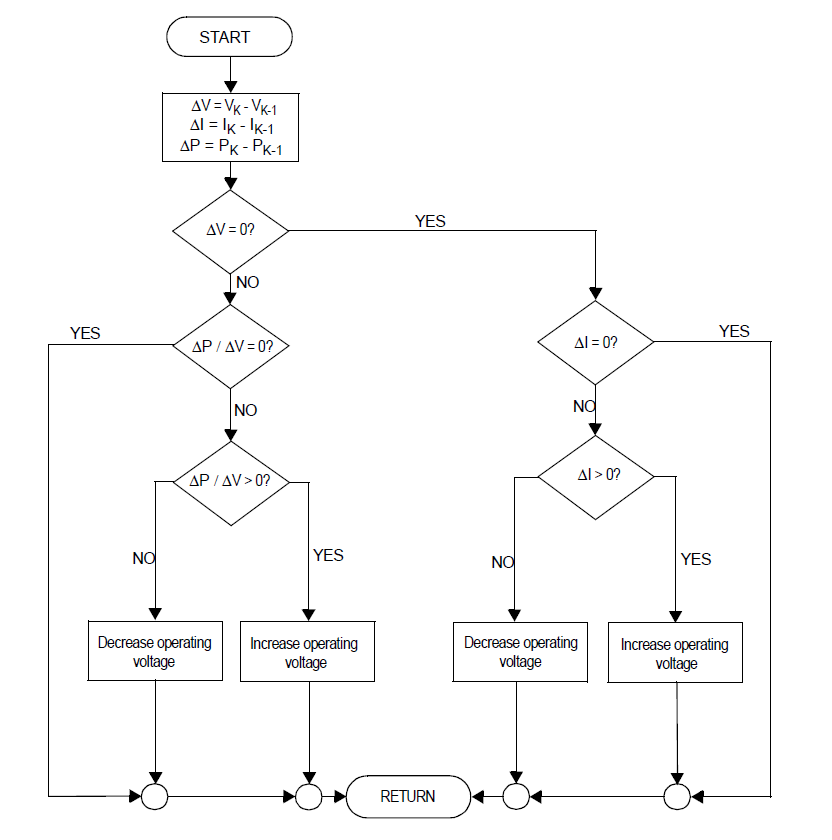
\includegraphics[width=0.7\textwidth]{../Pictures/P1/Flow_chart/flow_chart_incremental_conductance}
		\caption{flow chart incremental conductance \cite{AN1521_MC} }
		\label{fcinccon}
	\end{center}	
\end{figure}
\todo{also a bit small of a figure, the text should be around the same size of the rest of the words i would say. AT}

